\part{Cours Magistral 6 -- Les intégrales}
\section{Rappel}

Théorème de Green

\begin{center}
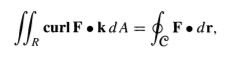
\includegraphics[scale=0.7]{image1.png}\\
\end{center}

où k = $\hat N$ et $kdA = dS$
Le théorème de Green fait le lien entre l'intégrale de surface et l'intégrale d'un contour fermé.


\section{Théorème de Stokes}

C'est une généralisation du théorème de Green

Nous avons une surface orientable par un vecteur normal.

\[\iint_S rot F\bullet \hat N dS = \oint F\bullet dr\]
\textit{Pour la démonstration, voire Adams page 914}

Ce théorème va nous donner un sens au $rot F$.

On trace un cercle de centre P et de rayon $\epsilon \to 0$ On peut appliquer le théorème.

\[\iint_{S_{\epsilon}} rot F\bullet \hat N dS = \oint_{C_{\epsilon}} F\bullet dr\]

Or on a que
\[\iint_{S_{\epsilon}} rot F\bullet \hat N dS = rot F (P) \bullet \hat N (P) \iint_{S_{\epsilon}} dS\]

Et \[\iint_{S_{\epsilon}} dS\] est l'aire du disque. C'est à dire $\pi \epsilon ^2$

\[\Rightarrow rot F(P) \bullet \hat N = \lim_{\epsilon \to 0 }\frac{1}{\pi \epsilon ^2} \oint_{C_{\epsilon}}F\bullet dr\]

Que veut dire le nom "rotationnel" ?

Prenons un champ de vecteur
\[\vec F = \vec v = x \vec j +0 \vec i +0 \vec k\]

C'est la cinématique d'un écoulement de cisaillement. Nous avons un matérau fixe ainsi qu'un matériau qui avance à côtés.
Si on place une "boule" dans ce champ vectoriel, la boule va monter et elle va également avoir un mouvement de rotation tout à fait fictif. Il a un lien avce le rotationnel. Dans ce cas-ci,\[rot \vec v = \vec k\]

Il est perpendiculaire au plan et il est constant.

Faisons donc le lien entre le rotationnel d'un champ de vecteur et la vitesse angulaire de rotation locale en un point P ( de la boule citée plus haut ).

On considère le point


$P = ( r \cos \Theta, r \sin \Theta ) \vec r $

On peut trouver

\[ v = r^{\bullet} = (-r\sin \Theta \Theta^{\bullet}, r\sin \Theta \Theta^{\bullet}\]

\[v = (-y \Omega , x \Omega) \]

\[v=(-y\Omega) i + (x\Omega) j \] est la rotation de corps rigide à vitesse angulaire $\Omega$

Faisons comme si on n'avait pas le Théorème de Stokes. Calculer la criculation de v le long de $C_{\epsilon}$

$$r^{\thicksim} = (x_0+ \epsilon \cos t ) i +( Y_0 + \epsilon \sin t )j $$

pour $\Theta \le t \le 2 \pi $

On dérive pour trouver

\[\frac{d r^{\thicksim} }{dt} + ( -\epsilon \sin t ) i + ( \epsilon \cos t ) j\]

On arrive donc à

\[\oint_{C_{\epsilon}} v \bullet dr^{\thicksim} = \oint_{C_{\epsilon}} ( v \bullet \frac{dr^{\thicksim}}{dt} ) dt \]


On calcule tout ça

\[\int_0^{2\pi} \left[ (-\Omega ( x_0 + \epsilon \sin t )) ( - \epsilon \sin t ) + (\Omega ( x_0 + \epsilon \cos t))( \epsilon \cos t ) \right] dt \]

Où

$-\Omega ( x_0 + \epsilon \sin t ) = V_x$



$- \epsilon \sin t  = \dfrac{dx}{dt}$



$(\Omega ( x_0 + \epsilon \cos t)) = V_y$




$\epsilon \cos t =\frac{dy}{dt}$




\[Circ = \int_0^{2\pi} (\Omega \epsilon ( y_0 \sin t + x_0 \cos t ) + \Omega \epsilon ^2 )\bullet dt \]

avec \[ \int_0^{2\pi} (\Omega \epsilon ( y_0 \sin t + x_0 \cos t )  = 0\]


\[Circ = \int_0^{2\pi} ( \Omega \epsilon ^2 )\bullet dt = \Omega \epsilon^3 ( 2 \pi ) = (\pi \epsilon^2 )\bullet ( 2 \Omega ) \]

\begin{myrem}
$rot v : ( 2 \Omega ) k = $ est un vecteur constant

On confirme bien stokes pour $\vec F = \vec V $


\[\iint_{S_{\epsilon}} rot v \bullet \hat N dS = \iint_{S_{\epsilon}} (2\Omega) k\bullet k dS = (2 \Omega ) \pi \epsilon ^2 = \oint_{C_{\epsilon}} v\bullet dr^{\thicksim} \]

\end{myrem}

\begin{myrem}


Dans ce exemple, la circ ne dépen pas de $(x_0,y_0)$ : car ici $ rot v = $ vecteur constant
\end{myrem}

\begin{myrem}

Il y a un sens à définir une vitesse angulaire locale au point P dans un fluide en mouvement à $\vec v$ comme étant

$$\vec \Omega (P) = 0.5 rot v (P) $$

Mécanique des milieux continus
\end{myrem}

\begin{myrem}
Dans l'exemple du début du cours, les lignes de courant sont rectilignes. En plus, elle va tourner et sa vitesse sera mesurée par le rotationnel.
\end{myrem}


Le théorème de Stokes est vraiment un outil fondamental des modèles de milieux continus ( macroscopiques ). Il permet aussi de calculer des intégrales compliquées.

On trace$C$, $S_1$, $S_2$ sont tous des bords d'une même surface.

\[\oint_C F \bullet dr = \iint_{S_1}rot F \bullet N dS = \iint_{S_2}rot F \bullet N dS\]
\textit{
Exemple : }

"Utiliser Stokes deux fois."

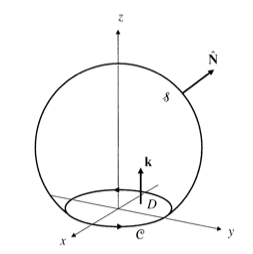
\includegraphics[scale=0.6]{image2.png}\\%Figure 16.17

C'est une sphère d'équation

\[x^2+y^2 + (z-2)^2 =8\] qui se trouve au dessus du plan ( x-y )

Le champ est le suivant
\begin{center}

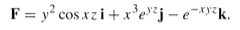
\includegraphics[scale=0.7]{image4.png}\\
\end{center}
Le vecteur normal doit être pris comme $\hat{\vec N} = \vec k $

On va prendre le disque qui forme la base de la sphère pour calculer l'intégrale. qui a pour équation $C : x^2 + y^2 = 4 $  et $S : x^2 + y^2 = 4 $ avec $S_2 \equiv 0 $


Il faut d'abord calculer le rotationnel de manière générale et puis on pose $z\equiv 0$

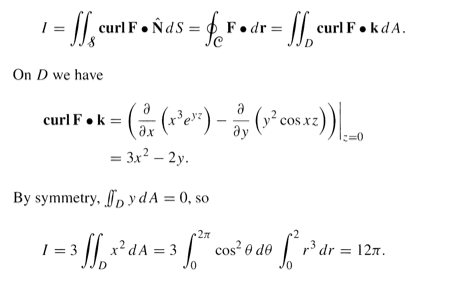
\includegraphics[scale=0.7]{image3.png}\\

\section{Théorème de la Divergence}
Ce théorème appartient à Gauss, Green, Ostrogradsky.

C'est un thèorème hyper fondamentale pour la suite.

S est une surface fermée orientée qui appartient à $\Re^3$

\[\iiint_D div F dV = \oiint_S F \bullet N dS\]
C'est une relation qui fait le lien entre une intégrale de volume de et de surface.
\textit{
Cas particulier : 2D}

\begin{center}
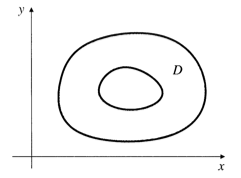
\includegraphics[scale=0.5]{image5.png}\\

\end{center}

\[\iint _R div F dA = \oint _C F \bullet N dS\]
C'est un cas particulier du thèorème de la divergence en 2D. On a pris une coupe d'un volume 3D.

\subsection{Intéprétation de div $\vec F$}

On considère une sphère de $\Re ^3$ de rayon $\epsilon \to 0$ centrée en P.

Ce qu'il va rester pour l'intégrale triple, c'est
\[div F(P) \dfrac{4\pi}{3} \epsilon^3 = \oiint _{S_{\epsilon}} F \bullet N dS \]

On voit donc que

$$div F (P) =  \lim_{\epsilon \to 0 } \frac{1}{\dfrac{4\pi}{3} \epsilon^3} \oiint _{S_{\epsilon}} F \bullet N dS $$

C'est le flux/ Volume

\subsection{Application du théorème de divergence}

\subsubsection{Calcul d'un flux}
\[\vec F = x i + y j + z k \]

Au CM4, nous avons calculer l'intégrale de flux à travers ce cylindre

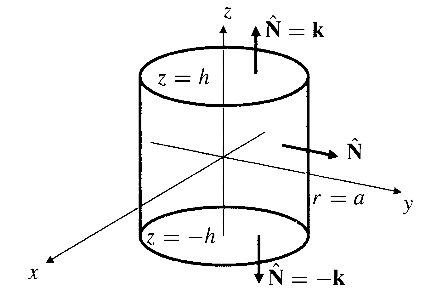
\includegraphics[scale=0.7]{image6.png}

On trouve donc

\[\iint_S F \bullet N DS = \iiint div f dV\]

On calcule donc

\[div F = \frac{\partial F_1}{\partial x}+ \frac{\partial F_2}{\partial y} + \frac{\partial F_3}{\partial z}= 1+1+1=3 = 3 \iiint dV = 6 \pi a^2 h\]

On avait obtenu la même chose au CM4

\subsubsection{Calculer $\oiint_S(x^2+y^2)dS$ sur la sphère S de rayon a centrée à l'origine}

\[x^2+y^2+z^2 = a^2\]

\begin{itemize}

\item Verifions s'il s'agit d'une intégrale de flux.

On a $\hat N = \dfrac{1}{a} r $

Or le vecteur position vaut
\[r = xi +yj +zk\]

On peut trouver
\[\dfrac{1}{a}r = \dfrac{1}{a}xi +\dfrac{1}{a}yj +\dfrac{1}{a}zk = \hat N\]

Il faut trouver F tel que $F\bullet \hat N = x^2 + y ^2 $

\[\Rightarrow F = axi +ayj +0k \]
\item Applique le théorème de la divergence

$$ I = \iiint_{Boule} div F dV = 2a \iiint_{Boule}dv$$

\[I = 2a \dfrac{4}{3}\pi a^3 = \dfrac{8}{3}\pi a^4\]
\end{itemize}

\begin{myrem}
Ne pas utiliser tel quel le Thèorème de la divergence si F n'est pas regulier dans D.


\emph{Exemple :} \[F = \dfrac{1}{||r||^3} r \] non régulier en r= 0

On établit un domaine $ D^* =D $ sans la boule centrée en 0 et puis on applique le théorème de la divergence à $D^*$

Voire Adams p910 ex 4
\end{myrem}

\begin{myrem}
\[\int_{C_{P_0 \to P_1}} \nabla f \bullet dr = f(P_1) - f(P_0) \]

\[\iint rot F \bullet dS = \oint F \bullet dr \]

\[\iiint div F dV = \oiint_S F \bullet DS\]

Ces trois théorèmes sont des généralisations des :


\[\int_a^b \frac{d}{dx}f dx = f(b) - f(a) \]

$\int$ dérivée de f = f aux bornes
\end{myrem}
